\documentclass[a4paper,11pt]{article}

\usepackage{url}
\usepackage{graphicx}
\usepackage{enumerate}
\usepackage{amsmath}
\usepackage{float}
\usepackage{longtable}
%\usepackage{fullpage}
\usepackage{pstricks}
\usepackage{tikz}
\usepackage[absolute]{textpos}
\usepackage{import}
\usepackage{subfigure}
\usepackage{setspace}

\title{G52CFJ C++ for Java Programmers \\ Coursework Documentation}
\author{Robert J. Golding (rjg08u)} \date{\today}

% Dutch style paragraph formatting
\setlength{\parskip}{1.3ex plus 0.2ex minus 0.2ex}
\setlength{\parindent}{0pt}

%\doublespacing
\onehalfspacing

\begin{document}
    \maketitle

    \section{Overview}

    The game is intended to be a clone of the popular Pacman game. Though it
    does not implement all of the functionality of the official game, all of
    the coursework requirements are fulfilled.

    \begin{figure}[ht]
        \begin{center}
            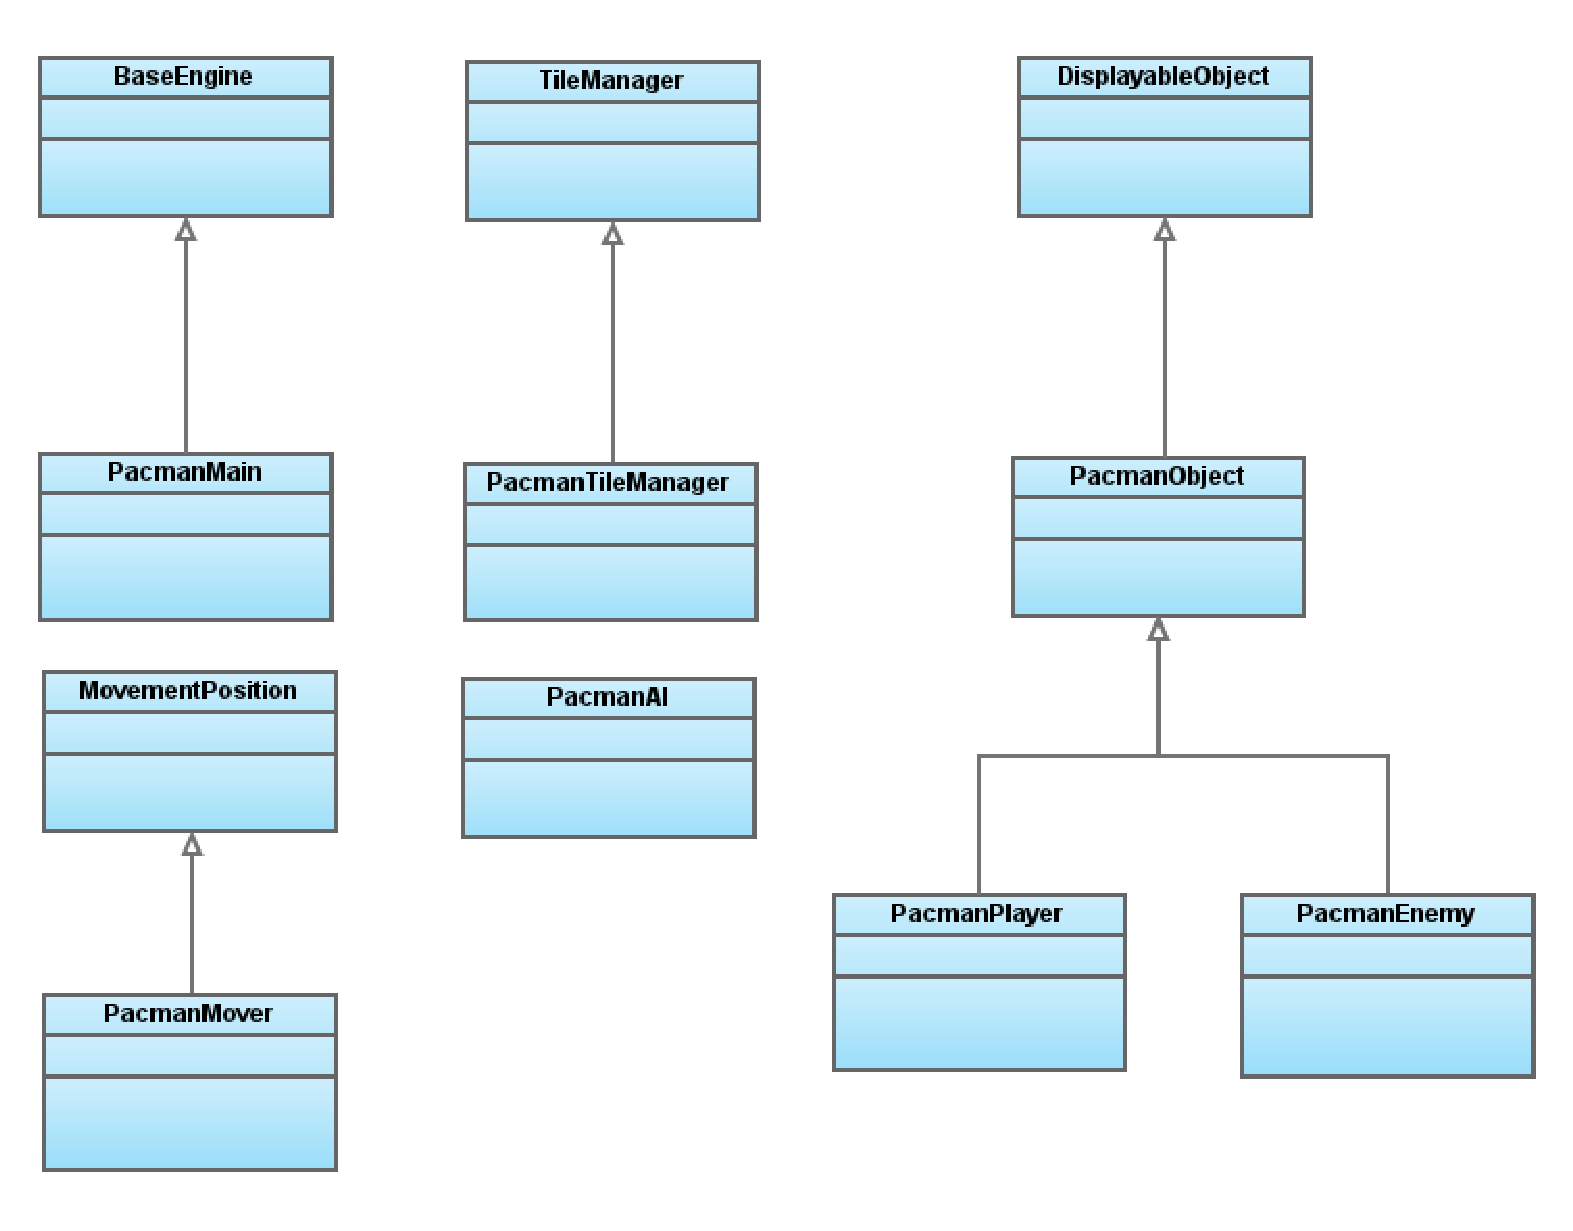
\includegraphics[width=\textwidth]{class-diagram}
        \end{center}
        \caption{Class diagram for the Pacman game}
        \label{fig:class-diagram}
    \end{figure}

    Figure \ref{fig:class-diagram} shows a class diagram of the game's objects
    for reference.

    \section{Usage}

    To start the game, compile it as normal and then run it with no arguments.
    The game will search the \verb!maps/! directory for any maps which will be
    loaded into the game in alphabetical order.

    The game starts with an initialisation screen, requiring the user to press
    the space bar to start. Once the game is running, pressing space again
    pauses. Pressing the escape key at any point exits the game.

    The aim of the game is to collect all of the ``pellets'' without being
    caught by the enemies. The larger pellets are ``power-ups'' which work in
    the same way as the original Pacman game---allowing the player to catch
    enemies, sending them back to their original starting location.

    Once all the pellets have been collected, the level is complete. Each
    pellet scores the player 10 points. A power-up pellet is worth 50 points.
    The power-up mode lasts for 5 seconds, and whilst in this mode normal
    pellets score double the normal amount (20 points).

    To move the player, use the arrow keys on the keyboard. Once moving, the
    player will continue to move in the same direction until a wall is reached,
    when it will stop. Pressing a key to move in a direction which is
    impossible due to a wall will delay that action until it is next available,
    in much the same way as the original Pacman game.

    \newpage

    \section{Requirements}

    \subsection{Draw an Appropriate Background}

    The background is drawn using the \verb!PacmanTileManager!, which is
    a subclass of the provided \verb!TileManager! class.

    The tile manager's state is loaded from the level's map file. There are
    5 types of tile in the game:

    \begin{itemize}
        \item Blank tile
        \item Wall
        \item Pellet
        \item Power-up
        \item Teleport
    \end{itemize}

    Pellets and power-ups can be collected by the player, and walls cannot be
    moved onto. Teleport tiles move the player to the opposite side of the
    screen (in the x-direction) if they are moved onto.

    \subsection{Have Moving Objects}

    The \verb!PacmanObject! class, which subclasses the provided
    \verb!DisplayableObject! class, provides an abstract moving object.
    \verb!PacmanPlayer! and \verb!PacmanEnemy! both inherit from this class,
    implementing their specific functionality.

    The player object is controlled by the keyboard, whereas the enemy objects
    are controlled by the AI. The enemies try to catch the player, and if they
    succeed the player loses a life.

    \subsection{Have Interaction Between the Objects \& Background}

    When the player moves onto a tile containing a pellet, a power-up or
    a teleport, an action is performed.

    When pellets are collected, the player's score is increased by 10 points
    (20 points in power-up mode). Power-ups cause the enemy objects to run away
    from the player, as the player can ``eat'' them. Also, the enemies change
    colour to signify to the user that they are scattering.

    \subsection{Provide User Interaction}

    The user controls the game entirely with the keyboard. The arrow keys
    control the direction of the player, which works in much the same way as
    in Pacman. The game can be paused by pressing the space bar.

    When life is lost the game requires the user to press the space bar to
    continue. The movable objects are reset to their original locations, but
    the background stays the same (so pellets which have already been collected
    are not reset).

    When a level is completed, the player must again press the space bar to
    continue---when the next map is loaded.

    \subsection{Provide AI-Controlled Objects}

    The enemy objects are controlled by a relatively simple AI algorithm. The
    AI is encapsulated in a separate class (\verb!PacmanAI!), which is provided
    to the enemy object on instantiation. This allows the AI algorithm to be
    swapped-out at runtime (i.e. the behaviour pattern).

    The AI determines which of the X or Y co-ordinates has a greater difference
    between the enemy and the player, and uses this information to move towards
    the player. The decision is weighted such that the enemy is more likely to
    go in the vertical (Y) direction.

    When in ``scatter'' (power-up) mode, the enemy's decisions are simply
    reversed. This has the effect of making the enemies run away from the
    player.

    \newpage

    \subsection{Load Data From Files}

    The map data is loaded from a file, with one file corresponding to each
    level. The file format is a grid corresponding to each tile, with the
    following characters:

    \begin{itemize}
        \item \verb! ! (space): blank tile
        \item \verb!.! (dot): pellet
        \item \verb!o!: power-up
        \item \verb!w!: wall
        \item \verb!t!: teleport
        \item \verb!e!: enemy
        \item \verb!p!: player (only one per map)
    \end{itemize}

    The maps are loaded from the \verb!maps/! directory within \verb!src!. Map
    file names are in the format \verb!level_%d.txt!, with the integer level
    number being 1-9. Two maps are provided with the game (\verb!level_1.txt!
    and \verb!level_2.txt!), though more can be added simply by creating more
    map files.

    \subsection{Save and Load Information}

    Requirement not currently fulfilled.

    \subsection{Display Status Information on the Screen}

    When in the ``main'' game state (i.e. the player is playing), the status
    bar at the top of the screen shows the following information: lives left,
    current level and number of points. This status information updates in
    real-time as the game is played.

    Also, when the game is in ``power-up'' mode, the enemies change colour.
    This is the only indication to the player (apart from the fact that they
    are running away!) When there is 2 seconds or less remaining in power-up
    mode, the enemies flash to ward the player that the time has almost
    expired.

    \subsection{Support Different States}

    The game has a number of states:

    \begin{enumerate}
        \item Initialisation: the player is required to press the space bar to
            begin playing the game
        \item Main: the game is being played by the player
        \item Power-up: the player has collected a power-up and the enemies are
            vulnerable
        \item Paused: the player has paused the game and is required to press
            the space bar again to un-pause it
        \item Level completed: the player has completed the level by collecting
            all the pellets, and is required to press the space bar to continue
            to the next level
        \item Game completed: the player has completed the last level in the
            game.
        \item Life lost: the player has been caught by an enemy and lost
            a life, and is required to press the space bar to continue
        \item Game over: the player has lost all their lives and the game is
            over
    \end{enumerate}

    \section{Additional Comments}

    The game has been constructed to obey design principles where appropriate.
    The \verb!PacmanObject! class contains an implementation for all the common
    functionality between the two objects in the game (\verb!PacmanPlayer! and
    \verb!PacmanEnemy!).
    
    Also, the \verb!PacmanEnemy! class uses an instance of \verb!PacmanAI! to
    decide how to move around the map. A subclass of this type could be used to
    implement a more advanced AI, which would alter the behaviour of the enemy
    object.

    One small feature worth noting is the ability of the player to reverse its
    direction without finishing its current movement.  This offers movement
    that is more similar to that of the original Pacman game, without resorting
    to a more complex architecture.

    If the user wishes to reverse the direction of their player object, the
    game calculates how much the current movement has progressed thus far, and
    reverses it. This is calculated within a subclass of the
    \verb!MovementPosition! class, called \verb!PacmanMover! (within the
    \verb!Reverse()! method), and results in a smooth reversal of direction.

    Also worth note is the modified game time used for this program. When the
    game is paused, time is still progressing---so when unpausing, objects
    ``jump'' to where they were next heading for (as specified by their
    ``mover'' object).
    
    To remedy this issue, the game uses a ``pause timer'', which is incremented
    on every tick when the game is in a state other than \verb!stateMain!. The
    game time can then be calculated by subtracting the pause timer from the
    original game time. For the implementation, see the
    \verb!GetModifiedTime()! method of \verb!PacmanMain!.

\end{document}
